\section{Background}
%------------------------------------------------

%\begin{enumerate}[noitemsep] % [noitemsep] removes whitespace between the items for a compact look
%\item First item in a list
%\item Second item in a list
%\item Third item in a list
%\end{enumerate}

\subsection{Elevated Plus Maze}

Initially conceived in 1955 by K. C. Montgomery, the elevated plus maze was a way to study the simultaneous feelings of curiosity and fear that rats experience when exposed to a new environment. \cite{Montgomery1955}

The elevated plus maze is a four-arm, raised platform in the shape of a plus sign. The maze consists of two enclosed arms and two open arms, perpendicular to the enclosed. \cite{Carter2010} It is one of the most widely used and validated tests for measuring the anxiety responses of rats under variety of conditions. \cite{Walf2007}

As a result of early experiments, it was found that the rodent tends to spend more time in the enclosed arms. The behaviour observed within these experiments is as a result of the approach/avoidance conflict when a rat is within a new environment. \cite{Lister1987} It was common to record the behaviour of the animal for 5 minutes, as it was found that after this time, rats would acclimatise to their environment and its behaviour would change. \cite{Komada2008}

\subsection{E-puck}

Developed by \citeauthor{epfl-epuck} at the Autonomous Systems Lab of \'{E}cole Polytechnique F\'{e}d\'{e}rale de Lausanne (EPFL), the E-puck (see Fig \ref{fig:epuck-pic}) is  an open source, two wheeled, differential robot measuring roughly 7cm in diameter. \cite{epfl-epuck}

\begin{figure}[H]
	\centering
	\begin{minipage}{.5\textwidth}
		\centering
		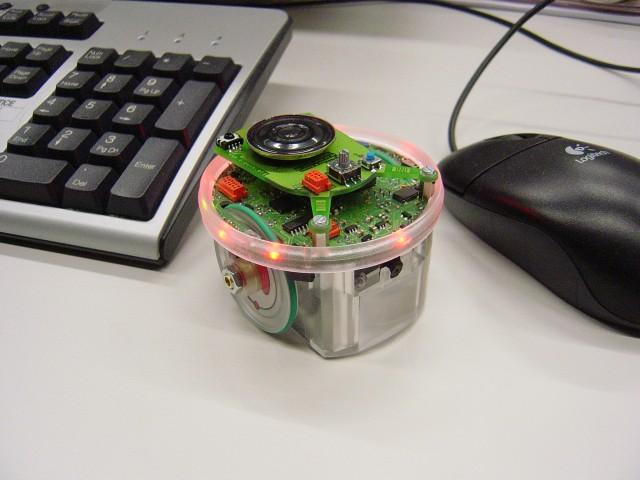
\includegraphics[width=.85\linewidth]{epuck}
		\captionof{figure}{E-puck mobile robot}
		\label{fig:epuck-pic}
	\end{minipage}%
\end{figure}

\begin{figure*}[!ht]
	\centering
	\def\layersep{2cm}
	\def\hiddenlayers{1}
	\def\hiddenneurons{2}
	
	\def\hiddenlayernodes{3}
	
	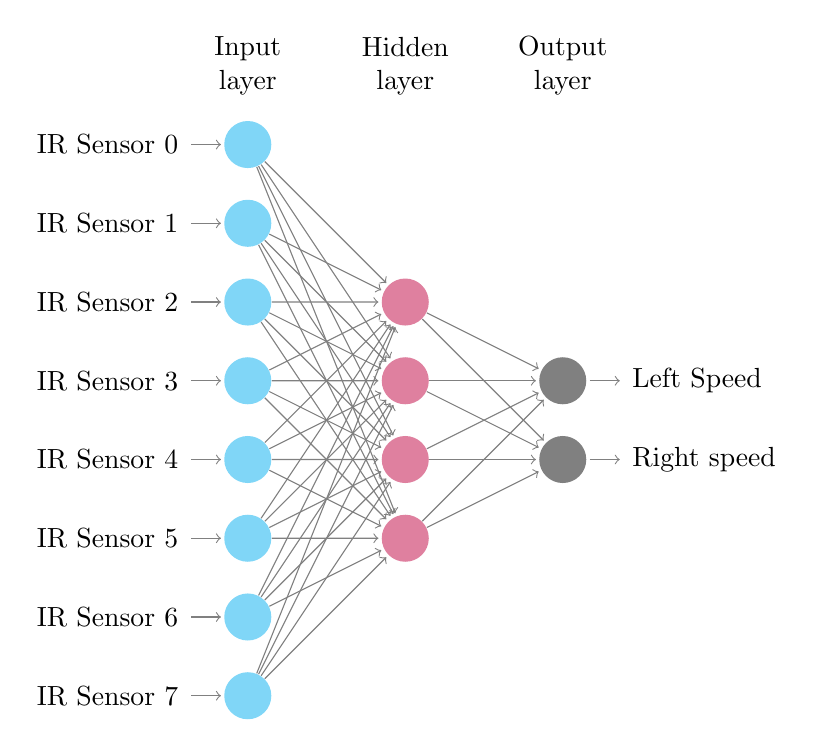
\begin{tikzpicture}[shorten >=1pt,->,draw=black!50, node distance=\layersep]
	\tikzstyle{every pin edge}=[<-,shorten <=1pt]
	\tikzstyle{neuron}=[circle,fill=black!25,minimum size=17pt,inner sep=0pt]
	\tikzstyle{input neuron}=[neuron, fill=cyan!50];
	\tikzstyle{output neuron}=[neuron, fill=black!50];
	\tikzstyle{hidden neuron}=[neuron, fill=purple!50];
	\tikzstyle{annot} = [text width=4em, text centered]
	
	% Draw the input layer nodes
	\foreach \name / \y in {0,...,7}
	% This is the same as writing \foreach \name / \y in {1/1,2/2,3/3,4/4}
	\node[input neuron, pin=left:IR Sensor \y] (I-\name) at (0,-\y) {};
	
	% Draw the hidden layer nodes
	\foreach \name / \y in {0,...,\hiddenlayernodes}
	\path[yshift=-2cm]
	node[hidden neuron] (H-\name) at (\layersep,-\y cm) {};
	
	
	% Draw the output layer node
	\node[yshift=0][output neuron,pin={[pin edge={->}]right:Left Speed}, right of=H-1] (O-1) {};
	\node[yshift=0][output neuron,pin={[pin edge={->}]right:Right speed}, right of=H-2] (O-2) {};
	
	% Connect every node in the input layer with every node in the
	% hidden layer.
	\foreach \source in {0,...,7}
	\foreach \dest in {0,...,\hiddenlayernodes}
	\path (I-\source) edge (H-\dest);
	
	
	% Connect every node in the second hidden layer with the output
	\foreach \source in {0,...,\hiddenlayernodes}
	\foreach \dest in {1,...,2}
	\path (H-\source) edge (O-\dest);
	
	% Annotate the layers
	\node[xshift=0cm][annot,above of=I-1] (first) {Input layer};
	\node[xshift=1cm][annot,right of=first, node distance=1cm] (hl) {Hidden layer};
	\node[xshift=1cm][annot,right of=hl, node distance=1cm] (ll) {Output layer};
	\end{tikzpicture}
	\caption{Neural network}
	\label{fig:NN}
\end{figure*}

The E-puck was originally developed to allow students to address a wide range of engineering fields. 

The platform features a wide range of sensing capabilities as standard, with the additional option to expand through the use of top and bottom extension slots. These physical extensions can range from extra sensors, to additional controllers for more computational capabilities (such as an Arduino board).

The E-puck has a multitude of sensors, including eight infrared proximity sensors, an accelerometer, microphones and a colour CMOS camera in front. Its actuators consist of two stepper motors which control the movement of the two wheels.

%The e-puck is a small (diameter 75mm) mobile robot designed for education in engineering by École polytechnique fédérale de Lausanne (EPFL). The robot structure is simple, being made of only four injected plastic parts: the main body, the light ring, and the two wheels (Fig. 2). The main body is the core of the mechanical structure and holds the battery. The main PCB is screwed on top of the main body. The e-puck has a multitude of sensors, including eight infrared proximity sensors, an accelerometer, microphones and a colour CMOS camera in front. Its actuators consist of two stepper motors which control the movement of the two wheels with a resolution of 1000 steps per wheel revolution (Mondada et al. 2006). In the implemented simulation, the eight proximity sensors as well a GPS module are used.

\subsection{Webots}

Webots is a commercial simulation software which supports the e-puck and includes libraries of sensors and actuators for creating and tailoring robot models. It allows for the creation of complex environments for the robot simulation and supports three-dimensional physics through the Open Dynamics Engine library.
 
It is quite advantageous to perform simulations prior to investigations with real robots. This is because simulations are faster, easier to set up and cheaper to use.

For example, a real robot is susceptible to damage from the environment, such as drops, liquid spills or is hit by an object. Repairing such damage could be costly, both in time and cost. However, within a simulation, this does not cost anything.

In this experiment's example, if a real robot was used, it would have to be fixed or replaced each time a controller failed. In addition to this, a genetic algorithm was used, and this would require a significant investment of time using a real robot microcontroller. \cite{Michel2004}

Despite this, the simulation results are transferable onto real robots. Therefore, once the best controller has evolved, this could be run on a physical e-puck.

The elevated plus maze was modelled in Webots. Our model is shown in Fig. \ref{fig:arena}, along with the E-puck model.

\begin{figure}[H]
	\centering
	\begin{minipage}{.5\textwidth}
		\centering
		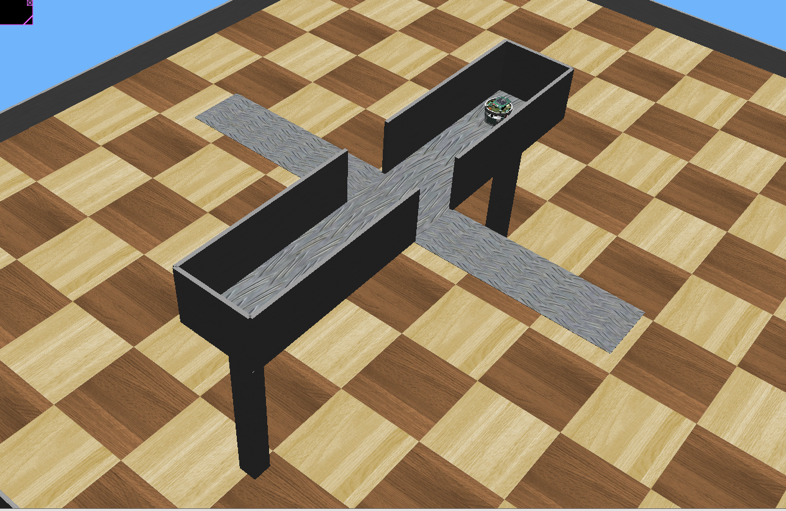
\includegraphics[width=.85\linewidth]{arena}
		\captionof{figure}{Simulation arena}
		\label{fig:arena}
	\end{minipage}%
\end{figure}

\subsection{Neural Network}

An Artificial Neural Network (ANN) is a system that is modelled on the biological brain, particularly on the hypothesis that mental activity consists primarily of electrochemical activity in networks of brain cells called neurons.

The signal output of a neuron can either cause excitation or inhibition in the neuron it is connected to. When a neuron sends an excitatory signal to another neuron, this signal is added to all of the other inputs of that neuron. If it exceeds a given threshold then it will cause the target neuron to fire an action potential, if it is below the threshold then no action potential occurs. \cite{Russell2009}

An ANN is comprised of nodes (neurons) connected by directed links. Each neuron receives input values either from the environment or from other neurons. Based on these inputs, the neuron calculates an output value by way of an activation function. Each link also has a numeric weight, known as a synaptic weight, associated with it, which determines the strength and sign of the connection. In effect, it is a distributed and parallel processor.

The network acquires knowledge from its environment through a learning process; a learning algorithm. The objective is to modify the network’s synaptic weights for the network to perform its desired function. The ability for synapses to modify is known as synaptic plasticity. \cite{Haykin2008}

Shown in Fig. \ref{fig:NN} is the utilised network.


\subsection{Genetic Algorithm}

A genetic algorithm is an iterative optimisation method based on natural selection that attempts to emulate the process of biological evolution. \cite{Fraser1970}

The algorithm begins by first creating a random set of possible solutions to the problem.

Each solution is called an \textit{individual} with its properties being termed \textit{chromosomes}. These chromosomes contain \textit{genes} and the complete set of possible solutions is the \textit{population}. 

Each individual in the population is evaluated based on how well it performs as a solution to the problem according to a fitness function. 

The result of this fitness function is a performance metric for the individual, and a selection operator utilises this metric to select individuals to create the next generation, a method termed \textit{reproduction}.

This is achieved through a genetic operator called a crossover, which is the mixing of a certain number of traits (genes) from each parent to produce an offspring. After this, random mutation of individuals in the population may occur. The algorithm terminates when a certain number of generations has been produced or when a solution with an acceptable level of fitness has been found. 

